\appendixpageoff
\begin{appendices}
\chapter{The system usability scale standard version}
\begin{figure}[ht!]
  \centering
  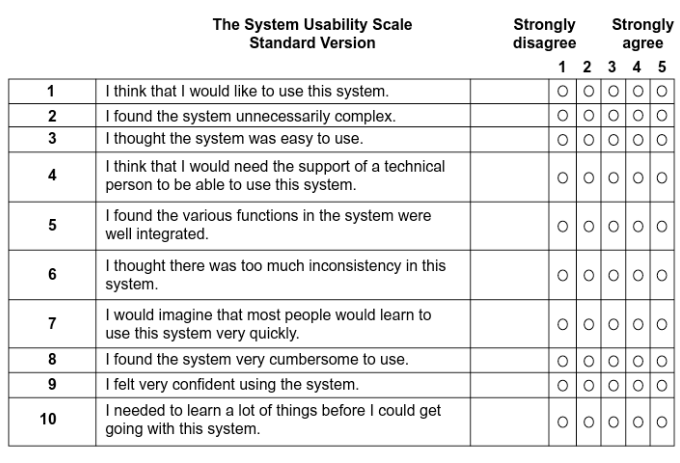
\includegraphics[width=\textwidth]{Images/SUS.png}
  \caption{the SUS}
  \label{architectureOverview}
\end{figure}
The image above was downloaded from \cite[susImage]. It represents the SUS graphically. It is evaluated as the sum of all the answers multiplied by 2.5 and then divided by the number of participants. If the gotten value is higher than 68 the usability of the system is above average. This is approach is a rough estimate on how a system is usable.
The mathematical averages of the answers to each item of our participants were the following: 
\lstset{style=sharpc, numbers=left}
\begin{lstlisting}
	4
	1.2
	4
	1.4
	3.6
	1.6
	4.4
	2.4
	3.2
	1.6
\end{lstlisting}
After applying said technique to get the result of the usability of KenticoApp we got the number 68.5. 

\chapter{How to start using KenticoApp}
\begin{description}
\item[1.] The user has to enable the installation of Android package kits (APK) outside of Google Play on his mobile device
\item[2.] The APK has to be installed and launched
\item[3.] To be able to use KenticoApp the user has to have Internet connection
\item[4.] The username to be able to sign into KenticoApp is \textit{Test} and the password is \textit{admin}
\end{description}
\end{appendices}